\section{Predicate Exchange}
To condition a model $\cM$ on a predicate $Y$ we develop Predicate Exchange, a likelihood-free inference procedure.  It is composed of two parts:
\begin{enumerate}
\item \textbf{Predicate Relaxation} constructs a relaxed predicate $U_Y$ from $Y$. $U_Y$ takes values in the unit interval $[0, 1]$ rather than $\{0, 1\}$.
$U_Y$ is 1 iff $Y$ is 1, but otherwise takes nonzero values denoting the degree to which $Y$ is satisfied.
% The relaxation is parameterized by a temperature.
% Predicate relaxation allows us to apply likelihood based MCMC inference procedures.
\item  \textbf{Replica Exchange} is a Markov Chain Monte Carlo proecdure that exploits temperature. The degree to which $U_Y$ relaxes $Y$ is modulated by a temperature parameter $\alpha$, which trades off between accuracy and ease of inference.  By simulating several replicas of $U_Y$ at different temperatures, replica exchange is able to draw exact samples. 
\end{enumerate}

\subsection{Predicate Relaxation}

A relaxed predicate $U_Y$ is an approximation of $Y$ in the sense that WHAT?
There are three desiderata which govern this approximation.
First, $U_Y$ should have a temperature parameter $\alpha$ that controls the fidelity of the approximation. In particular, $U_Y$ should converge to $Y$ as $\alpha \to 0$, and to a flat surface as $\alpha \to \infty$. Second, the fidelity of the approximation should vary monotonically with temperature. Third, $U_Y$ should be consistent with $Y$ on 1. That is $Y(\omega) = 1$ iff $U_Y(\omega) = 1$ at all temperatures.  


% The family of approximations of the predicate $Y$ is parameterized through a temperature $\alpha$ that controls the smoothness of the approximation. In particular, $U_Y$ with $\alpha \to 0$ converges to $Y$ itself while increasing values of $\alpha$ yield smoother approximations eventually giving a flat surface when $\alpha \to \infty$. Moreover, the set of conditional samples $C(Y) = \{ \omega \in \Omega \text{ } | \text{ } Y(\omega) = 1 \}$ are assigned a value of $1$ in $U_Y$ for all temperatures. 

% To construct a $U_Y$ with such properties, we let $Y$ be the following predicate $a=b$ for standard Gaussians $a, b \sim \mathcal{N}(0, 1)$. We choose a distance
% $\rho(a, b)$ to indicate how close our sample is to $C(Y)$. To meet the desiderata
% of having $C(Y)$ be $1$ over the constraint set and to ensure the constraint becomes
% smoother with large $\alpha$, we use a function $k : [0, \infty] \to [0, 1]$ parameterized by $\alpha$ to wrap the distance $\rho(a, b)$. A simple choice for such a function is $k(d; \alpha) = e^{-d / \alpha}$ that provides the desired properties to $U_Y$ (see Appendix). The formal definition of $U_Y$ is as follows.

\begin{definition}
The function $U_Y : \Omega \to [0, 1]$ parameterized by $\alpha \in [0, \infty)$ is a relaxation of a $Y: \Omega \to \{0, 1\}$ if:
\begin{enumerate}[label=(\roman*)]
	\label{def:temp}
	\item For all $\omega \in \Omega$, $\lim_{\alpha \to 0}U_Y(\omega; \alpha) = Y(\omega)$.
	\item For all $\omega \in \Omega$, $\lim_{\alpha \to \infty}U_Y(\omega; \alpha) = 1$.

    \item For all $\alpha$, $U_Y(\omega; \alpha) = 1$ iff $Y(\omega) = 1$.
    \item The entropy $H(U_Y(\omega; \alpha))$ (which characterizes the fidelity of the approximation ) is an increasing function of $\alpha$.\footnote
    {By compactness, it is integrable for all $\alpha$, when $\Omega$ has finite dimension}
\end{enumerate}
\end{definition}


The construction of $U_Y$ from $Y$ (Section \ref{implement}) substitutes primitive predicates (equality, inequalities and logical operators) in the model with soft predicates Figure \ref{softpreds}.  Soft predicates rely on a notion of distance, such that the degree to which a predicate is satisfied is a measure of closeness in a metric space. 
For example if $x$ and $y$ are real values, then $x \soft{=} y$ is defined as $k_\alpha(\rho(x, y))$ where $\rho$ is a distance function and $k$ is a relaxation kernel paramterized by temperature $\alpha$.
A relaxation kernel maps distances to values in $[0, 1]$.
Examples are given in Figure \ref{kernels}.
If the squared exponential kernel is used for example then $x \soft{=} y = \exp(\norm{x - y}/\alpha)$.

\begin{figure}\label{kernels}
\begin{align*}
k_{SE}(r) &= \exp\left(-\frac{r^2}{\alpha}\right) & \text{Squared Exponential}\\
k_{SE}(r) &= \sigma^2\left(1 + \frac{r^2}{2 \alpha \ell^2}\right)^{-\alpha} & \text{Rational Quadratic}
\end{align*}
\caption{Relaxation Kernels}
\end{figure}

The relaxation of an inequality such as $x > y$ relies on the amount by which $x$ must be increased (or $y$ decreased) until $x > y$ is true.
This is the distance between $x$ and the interval $[y, \infty]$, where the distance between a point and any interval $[a, b]$ is the smallest distance between $x$ and any element in $[a, b]$ (and therefore 0 if $x \in [A, b]$:
\begin{equation}
\rho(x, [a, b]) =
\begin{cases}
  a - b, & \text{ if } x < a\\
  x - b, & \text{ if } x < b\\
  0,              & \text{otherwise}
\end{cases}
\end{equation}

In general, a distance metric on points extends naturally to sets:
\[
\rho(x, A) = \inf \left\{\rho(x, a) \mid a \in A\right\}
\]


  % \begin{center}
  % \begin{tabular}{ c |  c | c }
  %   \hline		
  %   $x \soft{=} y$ & $x \soft{>} y$ & $x \soft{<} y$  \\
  %   $k_\alpha(\rho(x, y))$ & $k_\alpha(\rho(x, [y, \infty]))$ & $k_\alpha(\rho(x, [-\infty, y]))$ \\
  %   \hline  
  % \end{tabular}
  % \end{center}


\begin{figure}\label{softpreds}
  \begin{align*}
x \soft{=} y &= k_\alpha(\rho(x, y))\\
x \soft{>} y &= k_\alpha(\rho(x, [y, \infty]))\\
% x \soft{<} y &= k_\alpha(\rho(x, [-\infty, y]))\\
x \soft{<} y &= k_\alpha(\rho(y, [-\infty, x]))\\
a \soft{\land} b &= \max(a, b)\\
a \soft{\lor} b &= \min(a, b)
  \end{align*}
\caption{Soft Primitive Predicates}
\end{figure}

\paragraph{Negation}
Soft Negation is a necessary of a complete Boolean algebra, but introduces complications.
In Figure \ref{negationimg}(A), shows $x \soft{>} 0$ as a function of $x$.
The standard \cite{} approach to negation of $a \in [0, 1]$ is $1 - a$.
However, as shown in Figure \ref{negationimg} (b) this violates criteria (iii) of predicate relaxation.
That is, there are values which satisfy the hard predicate $\neg(x > 0)$ which do take a value of 1 in $1 - (x \soft{>} 0)$.
Ultimately this would cause inference using soft predicates to be incorrect.

\begin{figure}
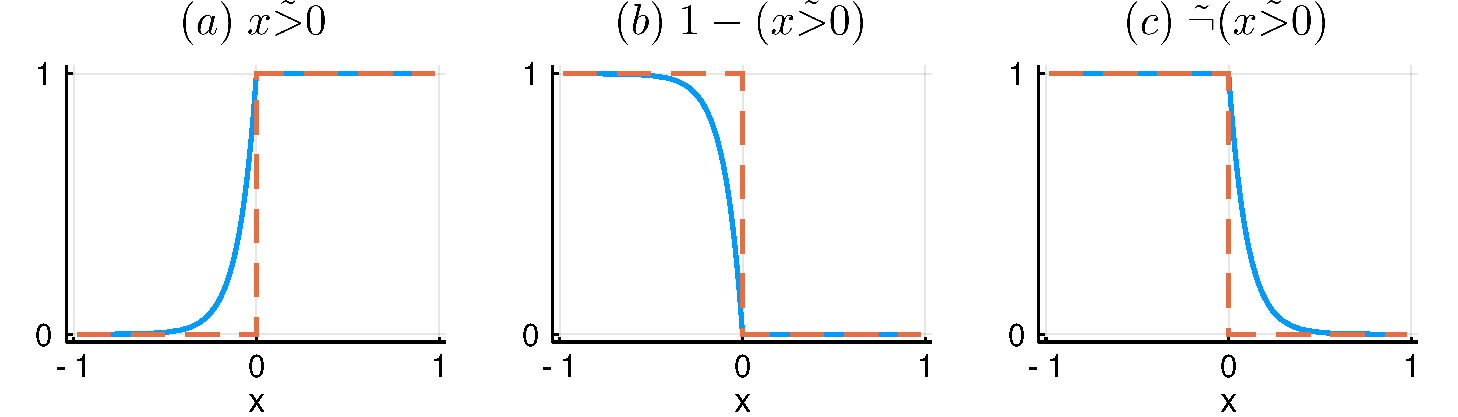
\includegraphics[width=\linewidth]{negation.pdf}
\caption{Soft predicates as function of $x$.  In all figures the blue line denotes the soft predicate, while the red line denotes the predicate to approximate.}\label{negationimg}
\end{figure}


The problem arises because $U_Y$ as defined preserves consistency with $Y$ at 1 but not at 0.
In other words, $U_Y$ is a one-sided approximation.
To overcome this challenge we construct two-sided approximations.
For models where negation is used, a two-sided relaxed predicate yields a pair $(b_0, b_1)$, where $b_0, b_0 \in [0, 1]$.
$b_1$ preserves consistency with $Y$ on $1$, just as before, whereas $b_0$ preserves consistency with $\neg Y$ on $1$ (or equivalently $Y$ on 0).
For example if $x \dsoft{>} 0 = (b_0, b_1)$, then as a function of $x$, $b_0$ and $b_1$ correspond to Figure \ref{negationimg}(a) and (c) respectively.

A complete two-sided soft logic is shown in Figure \ref{softw}.
 
\begin{definition}
The function $U_Y : \Omega \to [0, 1]^2$ parameterized by $\alpha \in [0, \infty)$ is a two-sided relaxation of a $Y: \Omega \to \{0, 1\}$ if:
\begin{enumerate}[label=(\roman*)]
	\label{def:temp}
	\item For all $\omega \in \Omega$, $\lim_{\alpha \to 0}U_Y(\omega; \alpha) = (\neg Y(\omega), Y(\omega))$.
	\item For all $\omega \in \Omega$, $\lim_{\alpha \to \infty}U_Y(\omega; \alpha) = (0, 1)$.

    \item For all $\alpha$, $U_Y(\omega; \alpha) = 1$ iff $Y(\omega) = 1$.
    \item The entropy $H(U_Y(\omega; \alpha))$ (which characterizes the fidelity of the approximation ) is an increasing function of $\alpha$.\footnote
    {By compactness, it is integrable for all $\alpha$, when $\Omega$ has finite dimension}
\end{enumerate}
\end{definition}


\begin{figure}\label{softw}
\begin{align*}
x \dsoft{=} y &= (\text{if } x = y  \text{ then } \alpha \text{ else } 1, k_\alpha(\rho(x, y)))\\
x \dsoft{>} y &= (k_\alpha(\rho(x, [-\infty, y])), k_\alpha(\rho(x, [y, \infty])))\\
x \dsoft{<} y &= (k_\alpha(\rho(y, [x, \infty])), k_\alpha(\rho(y, [-\infty, x])))\\
(a_0, a_1) \dsoft{\land} (b_0, b_1) &= (a_0 \soft{\land} b_0, a_1 \soft{\land} b_1)\\
(a_0, a_1) \dsoft{\lor} (b_0, b_1) &= (a_0 \soft{\lor} b_0, a_1 \soft{\lor} b_1)\\
\dsoft{\neg}(a_0, a_1) &= (a_1, a_0)
\end{align*}
\caption{Soft Primitive Predicates with Two-Sided Error}
\end{figure}

% \begin{center}
% \begin{tabular}{ l | c | r }
%   % \hline		
%   $(a_0, a_1) \soft{\land} (b_0, b_1)$ & $(a_0, a_1) \soft{\lor} (b_0, b_1)$ & $\neg(a_0, a_1)$ \\
%   $(a_0, a_1) \soft{\land} (b_0, b_1)$ & $(a_0, a_1) \soft{\lor} (b_0, b_1)$ & $\neg(a_0, a_1)$ \\
%   % \hline  
% \end{tabular}
% \end{center}



\subsection{Approximate Markov Chain Monte Carlo}
A relaxed predicate can serve as an approximate likelihood in likelihood based inference methods such as Markov Chain Monte Carlo.
MCMC algorithms require a function $f$ that is proportional to the the target density.
In Bayesian inference this is the posterior, dictated by Bayes' theorem as the product of the likelihood and the prior.
Approximate inference using relaxed predicates takes a similar form.

Let $\cM$ be a model, $Y$ be a predicate that conditions $\cM$, and $U_Y$ be a relaxation of $Y$.
% Random variables in $\cM$ may be exogenous or endogenous in the sense that
% given values for exogenous variables, the values of endogenous are determined.
% For example $X = \mathcal{N}(0,1)$ is exogenous while $Y = X^2$ is endogenous.
% Inference need only take place on exogenous random variables.
Both $Y$ and $U_Y$ are random variables, and hence map from the sample space $\Omega$.
For convenience it is useful to define a soft predicate as a function of its parameters, i.e., other random variables in the model.
Let $u$ denote a relaxed predicate that takes as input values of random variables in the model, rather than elements of the sample space.
That is, if $X_1(\omega), \dots, X_n(\omega) = x_1, \dots, x_n$, then $u(x_1, \dots, x_n) = U_Y(\omega)$.
Assuming a prior density $p$, the approximate posterior $f$ is the product:
\begin{equation}
f(m) = p(m) \cdot u(m)
\end{equation}
$u$ effectively down-weights values of parameters which violate the predicate the model is conditioned on by the  degree to which they violate the predicate. 
This is modulated by temperature.  zero temperature $f$ recovers posterior exactly, since parameter values which violate the condition are given zero weight.

For illustration, let $\cM = (\mu, X_1, X_2)$ be a model where $\mu = \mathcal{N}(0, 1), Y \mathcal{N}(\mu, 1)$, $X_2 = X_1^2$ and $\cM$ is conditioned on $X_2 = 1$.
Since $X_2$ is a pure function of $X$ (i) and (ii) we can exclude it for inference.
The approximate posterior is shown at different temperatures in Figure \ref{temppost} and defined as:

$$
f(x, y) = \mathcal{N}_{0,1}(x) \cdot \mathcal{N}_{0,1}(y) \cdot k(x + y, 0) 
$$

\begin{figure}\label{temppost}
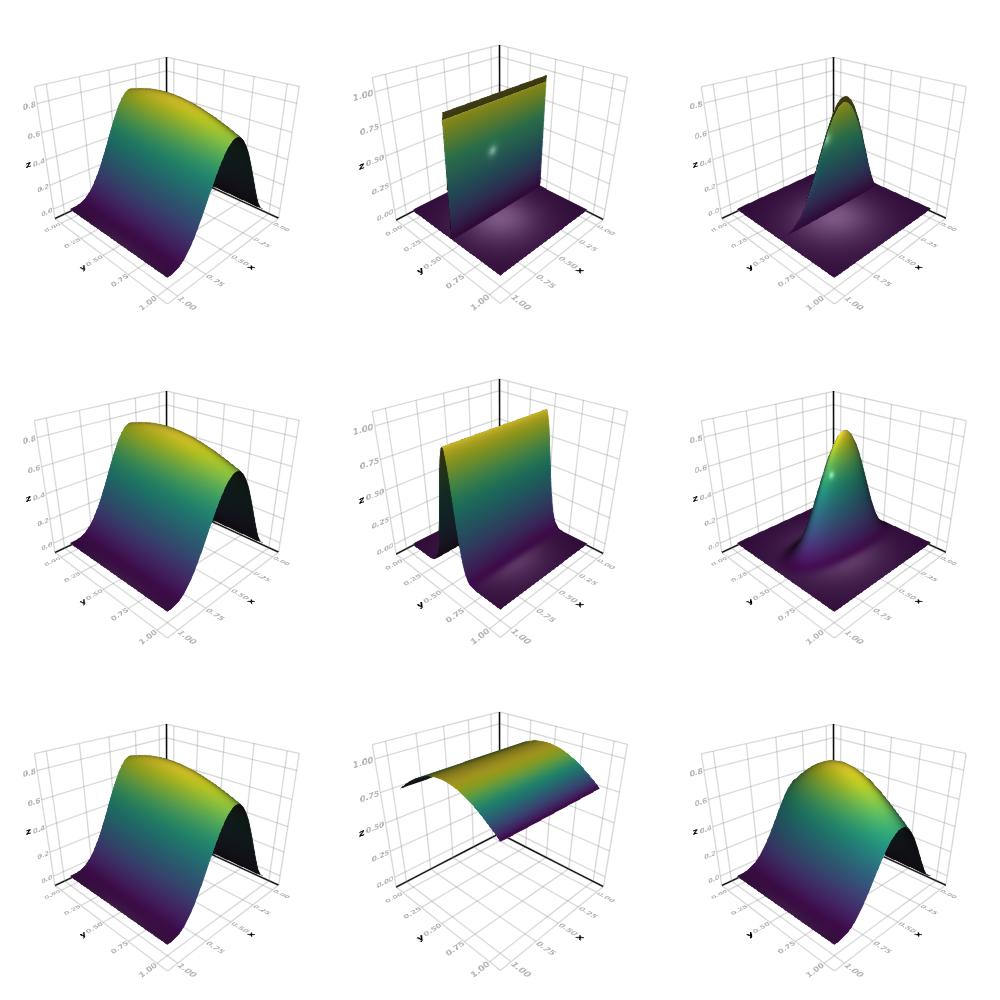
\includegraphics[width=\linewidth]{approxpost.png}
\caption{Approximate Posterior at varying temperatures}
\end{figure}



\subsection{Replica Exchange}

The temperature parameter trades off between tractability of inference and the fidelity of the approximation.
Too high and $U_Y$ will diverge too greatly from $Y$; too low and convergence will be slow.
% Several temperatre methods for controlling temperature exist such as simulated annealing \citep{kirkpatrick1983optimization} and Adiabatic Monte Carlo \citep{betancourt2014adiabatic}.
Replica exchange (also known as parallel tempering) \citep{swendsen1986replica} combines information from several chains to more  effectively sample from the zero temperature chain.

In a replica exchange, we simulate $M$ replicas at different temperatures, and periodically swap the temperatures of chains according to a predefined schedule.
Replica exchange uses a Metroplis-Hastings update to swap between changes while preserving the target distribution.

Assuming w.l.g that there are have two independent, parallel chains with targets $f(x)$, $g(y)$ and hence joint target $\pi(x,y)=f(x)g(y)$.
Replica exchange exchanges states between the two chains while preserving the joint target.
That is, we propose a swap of $x$ and $y$: to move from $(x, y)$ to $(x^\star,y^\star)$, where $x^\star=y$ and $y^\star=x$.
The swap is accepted with probability $\min(1, A)$ where:
$$
A = \frac{\pi(x^\star,y^\star)}{\pi(x,y)} = \frac{\pi(y,x)}{\pi(x,y)} = \frac{f(y)g(x)}{f(x)g(y)}.
$$

In predicate exchange, $f$ and $g$ correspond to two approximate posteriors (Equation ) at different temperatures.
Since swapping states is equivalent to swapping predicates.

Replica exchange has a number of hyper-parameters: the number of parallel chains, the corresponding temperatures, the swapping schedule.
Several good practices are outlined in Following \cite{earl2005parallel}.  In practice, we logarithmically spaced temperature between $0$ and an upper bound, and swap adjacent chains (chain $1$ with $2$, $2$ with $3$, etc) periodically.

Replica exchange is relies on an inner MCMC algorithm to simulate the individual parallel chains.
For finite dimensional contonuous models we use the No U-Turn Sampler \cite{hoffman2014no}, a variant of Hamiltonion Monte Carlo.



% This scenario closely resembles the reparameterization trick \citep{Kingma:2014, rezende2014stochastic} where one resorts to include all the uncertainty of a random variable $z$ in a simple, easy-to-sample, parameter-free noise source such as $\epsilon \sim \mathcal{N}(\mathbf{0}, I)$. The actual random variable $z$ is then obtained through a parametric transformation of the noise, $z = f(\epsilon; \theta)$. Both methods separate the 
% uncertainty of a random variable from the deterministic transformation that results in a complex density. However, in the reparameterization trick the noise source is constant and controlled while the parametric transformation is meant to infer the structure of the resulting random variable. Conversely, our forward model -- deterministic transformation -- is constant and controlled, hence we simply transfer our inference problem to a much simpler space of $\Omega$.

% Predicate Exchange has a connection to approximate Bayesian computation (ABC) methods~\citep{beaumont2002approximate} in that ABC methods 
% sample using a distance function to induce a data likelihood. Our method differs in that conditionals can be any predicate not just
% one for an observed random variable.
% Finally for inference, with the soft predicates we define, we
% can use modern likelihood-free variational inference algorithms
% that construct an approximation to a conditional with only samples
% from the joint and samples from the conditional approximation~\citep{tran2017hierarchical}.

